%% AAAI 2026 — INFO-H410 Project Report
%% ARM32 Instruction Scheduler for Masked Cryptography
%% Compile: pdflatex main.tex (twice for references)

\documentclass[letterpaper]{article}

%% ---------- AAAI 2026 Required Packages ----------
\usepackage{aaai2026}          % Official AAAI 2026 style
\usepackage{times}
\usepackage{helvet}
\usepackage{courier}
\usepackage{url}
\usepackage{graphicx}
\usepackage{amsmath}
\usepackage{amssymb}
\usepackage{booktabs}
\usepackage{multirow}
\usepackage{microtype}
\usepackage{xcolor}
\usepackage{subcaption}
\usepackage{colortbl}                    
\usepackage[most]{tcolorbox}              


\urlstyle{rm}
\frenchspacing
\setlength{\pdfpagewidth}{8.5in}
\setlength{\pdfpageheight}{11in}

\definecolor{bayesColor}{HTML}{1F77B4}
\definecolor{cspColor}{HTML}{FF7F0E}  
\definecolor{dqnColor}{HTML}{2CA02C}  
\definecolor{techGray}{HTML}{555555}  
\definecolor{techBg}{HTML}{F2F2F2}    

\newcommand{\approachA}{\textcolor{bayesColor}{\textbf{Approach A}}}
\newcommand{\approachB}{\textcolor{cspColor}{\textbf{Approach B}}}
\newcommand{\approachC}{\textcolor{dqnColor}{\textbf{Approach C}}}

\newcommand{\bayesHead}[1]{\paragraph{\textcolor{bayesColor}{#1}}}
\newcommand{\cspHead}[1]{\paragraph{\textcolor{cspColor}{#1}}}
\newcommand{\dqnHead}[1]{\paragraph{\textcolor{dqnColor}{#1}}}

\newtcolorbox{underhoodbox}[1][]{%
  enhanced, breakable,
  colback=techBg, colframe=techGray,
  boxrule=0pt, leftrule=2pt,
  arc=0pt, outer arc=0pt,
  left=6pt, right=4pt, top=4pt, bottom=4pt,
  title={#1},
  before skip=4pt, after skip=4pt,
}

\newtcolorbox{preferbox}[1]{%
  enhanced,
  colback=white, colframe=#1,
  boxrule=0pt, leftrule=3pt,
  arc=0pt, outer arc=0pt,
  left=6pt, right=4pt, top=3pt, bottom=3pt,
  before skip=3pt, after skip=3pt,
}

\nocopyright

\title{Side-Channel-Secure ARM32 Instruction Scheduling:\\
A Comparative Study of Search, CSP, and Reinforcement Learning}

\author{
  \textbf{Tajani Mohamed}\\
  \textbf{Brantegem Romain}
}

\affiliations{
  Université Libre de Bruxelles (ULB)\\
  INFO-H410 — Artificial Intelligence, 2025--2026
}

\begin{document}

\maketitle

%% ============================================================
\begin{abstract}
  Masked cryptographic implementations split secret data into multiple
  shares to resist power-analysis attacks.  However, a na\"ive compiler
  may schedule instructions manipulating different shares within a few
  cycles of each other, enabling Hamming-distance leakage to power
  traces~\cite{kocher1999}.  We formulate ARM32
  instruction scheduling as both a combinatorial optimisation
  and a probabilistic risk-assessment problem. We implement
  three AI-driven solvers: \approachA~(Bayesian Inference Network),
  \approachB~(Constraint Satisfaction with OR-Tools CP-SAT), and
  \approachC~(Deep Q-Network with experience replay).
  Experiments across block sizes $n \in \{10, 30, 50\}$ show that CP-SAT
  consistently finds perfectly hard-constrained schedules, while the Bayesian
  approach gracefully degrades side-channel risk ($E[Leakage]$) probabilistically
  using a threshold $\tau$. Once trained, DQN schedules instructions in tens of milliseconds,
  yet its performance depends critically on both the reward
  calibration and the diversity of the training corpus.
\end{abstract}

%% ============================================================
\section{Problem Formulation}
\label{sec:problem}

\subsection{Background: Masking and Side-Channel Leakage}

Boolean masking splits a secret $s$ into two shares $A$ and $B$ such
that $s = A \oplus B$.  Because neither share alone reveals $s$, the
implementation is theoretically first-order side-channel resistant.
However, on an in-order pipeline (e.g.\ ARM Cortex-M3/M4), if an
instruction operating on share~$A$ is issued within $k$ cycles of one
operating on share~$B$, the processor register file may contain both
intermediates simultaneously, enabling Hamming-distance leakage to power
traces~\cite{kocher1999}.

\subsection{Formal Representation}

Let $\mathcal{I} = \{I_0, \ldots, I_{n-1}\}$ be a basic block of $n$
ARM32 instructions.  Each instruction carries:
\begin{itemize}\setlength\itemsep{0pt}
  \item \textbf{name}: ARM mnemonic (e.g.\ \texttt{EOR}, \texttt{LDR}).
  \item \textbf{dest\_reg}, \textbf{source\_regs}: register operands.
  \item \textbf{latency} $\ell_i \in \{1, 2\}$: pipeline latency
        (1 for ALU, 2 for MUL / LDR).
  \item \textbf{share\_type} $\sigma_i \in \{A, B, N\}$: cryptographic
        share affiliation (\textit{N} = neutral).
\end{itemize}

\paragraph{State space.}
A \emph{schedule} assigns a start cycle $t_i \ge 0$ to every
instruction such that:
\begin{align}
   & \text{(RAW)}  & t_j                                                                               & \ge t_i + \ell_i
   &               & \forall\, (i \to j) \in \mathcal{D}, \label{eq:raw}                                                  \\
   & \text{(SEC)}  & |t_i - t_j|                                                                       & \ge k
   &               & \forall\, i,j : \sigma_i \ne \sigma_j,\; \sigma_i, \sigma_j \ne N. \label{eq:sec}                    \\
   & \text{(SLOT)} & t_i                                                                               & \ne t_j
   &               & \forall\, i \ne j. \label{eq:slot}
\end{align}
$\mathcal{D}$ is the RAW (Read-After-Write) dependency graph extracted
from register operands.  The \emph{objective} is to minimise the
makespan $\max_i(t_i + \ell_i)$, equivalently minimising the number of
inserted NOPs.

\begin{underhoodbox}[Scheduling Problem]
  The scheduling problem is NP-hard in general~\cite{ullman1975}, its
  structure is bounded state space, hard constraints, stochastic latencies in
  real hardware.
\end{underhoodbox}

%% ============================================================
\section{Methodological Approaches}
\label{sec:methods}

\subsection{\approachA: Bayesian Network Inference}

We depart from rigid hardware-centric definitions of security distance and
model side-channel leakage as a probabilistic event using a Bayesian Network. Side-channel vulnerability is not binary; the risk
of Hamming-distance leakage between two cryptographic shares decays
as the temporal distance $\Delta t$ between their execution increases.

\paragraph{Network Model.}
The Bayesian Network predicts the boolean hidden variable $\text{Leakage}\ (L)$
using observed parent nodes:
\begin{enumerate}\setlength\itemsep{0pt}
  \item \textbf{Temporal Distance} ($\Delta t$): Pipeline cycles between executions.
  \item \textbf{Share Overlap}: Boolean tracking if instructions belong to different shares ($A$ vs $B$).
\end{enumerate}

\paragraph{Conditional Probability Tables (CPT).}
We define a physically-motivated heuristic CPT simulating pipeline capacitor discharge.
Given $\text{Share\_Overlap} = \text{True}$:
\begin{align*}
  P(L=1 \mid \Delta t=1)     & \approx 0.95 \\
  P(L=1 \mid \Delta t=2)     & \approx 0.50 \\
  P(L=1 \mid \Delta t=3)     & \approx 0.10 \\
  P(L=1 \mid \Delta t \ge 4) & \approx 0.00
\end{align*}
If $\text{Share\_Overlap} = \text{False}$, $P(L=1)=0$.

\paragraph{Scheduling Algorithm.}
The solver builds the schedule greedily. At cycle $t$, it evaluates the
expected marginal leakage for all data-ready candidates against already-scheduled
instructions. The candidate minimising this risk is selected. If the minimal
expected leakage among all candidates exceeds a strict Risk Threshold $\tau$ (e.g. 0.15),
the solver injects a \texttt{NOP}. This increments the cycle counter, naturally
increasing $\Delta t$ and decaying the Bayesian risk below $\tau$ for subsequent cycles.

\subsection{\approachB: Constraint Satisfaction (CSP)}

We lift the scheduling to a \emph{Constraint Satisfaction / Optimisation
  Problem} over integer variables $t_i \in [0, T_{\max})$, where
$T_{\max}$ is derived from a greedy warm-start schedule.  Constraints
(\ref{eq:raw})--(\ref{eq:slot}) are encoded directly.

\paragraph{OR-Tools CP-SAT backend.}  Since using external librairies is allowed, we prefered to
use Google OR-Tools
CP-SAT~\cite{ortools}, a SAT-based propagation engine instead of a custom implementation
that wouldn't have been as efficient for an NP-hard problem.
Each security-distance pair $(I_A, I_B)$ introduces a reification
Boolean $b$:
\begin{equation}
  (t_A - t_B \ge k) \cdot b \;\vee\; (t_B - t_A \ge k) \cdot (1-b).
\end{equation}
The makespan $\max_i(t_i + \ell_i)$ is minimised using the built-in
objective.  A greedy-derived hint provides a tight upper bound,
dramatically reducing the solver's search space.  CP-SAT exploits 4
parallel worker threads and delivers \emph{optimal} solutions for
$n = 50$ in typically under 1~s.

\begin{underhoodbox}[Under the hood]
  CP-SAT uses \emph{lazy-clause-generation}~\cite{ortools}, combining constraint programming with SAT solving techniques.
  Instead of generating all possible conditions upfront, it builds them on demand. When a contradiction is found, it uses \emph{Conflict-Driven Clause Learning} (CDCL) to deduce a new rule (clause) that prevents repeating the same mistake, drastically reducing the search space.
  Furthermore, it uses parallel workers running different strategies that share these learned rules, which explains why it solves complex instances like $n=50$ in under a second.
\end{underhoodbox}

\subsection{\approachC: MDP / Deep Q-Network}

We formulate scheduling as a Markov Decision Process:
\begin{itemize}\setlength\itemsep{0pt}
  \item \textbf{State $S$}: a 6-dimensional feature vector
        (remaining-instruction ratio, normalised cycles since last $A$
        and $B$ placements, ready-queue size, critical-path ratio,
        normalised current cycle).
  \item \textbf{Action $A$}: choose one ready instruction or issue NOP.
  \item \textbf{Default Reward}: $-1$ per cycle elapsed, $-10$ per security
        violation, $+50$ on completion.
\end{itemize}

The Q-function is a Multi-Layer Perceptron (MLP) that takes
$(\text{state features} \| \text{action features})$ as input and
outputs a scalar $Q$-value.  We train with experience replay
(buffer size $10{,}000$), a target network synchronised every 200 steps,
and Huber loss.  $\varepsilon$-greedy exploration decays from 1.0 to
0.05 at rate $0.997$ per episode.  GPU acceleration via PyTorch is used.

\paragraph{Stochastic training.}
Optionally, instruction latencies are perturbed by $\pm 1$ during
training with probability 0.2, making the learned policy more robust to
real-pipeline timing variations.

%% ============================================================
\section{Experimental Evaluation}
\label{sec:experiments}

\subsection{Setup}

First experiments were run over block sizes $n \in \{10, 30, 50\}$, three
random seeds (42, 43, 44), and security distances $k \in \{3, 50\}$.
For each $(n, k, \text{seed})$ tuple, the exact same instruction block is
given to all three solvers, ensuring a fair comparison.  The MDP is
trained for 5\,000 episodes on a single block.  All experiments run on a
single machine; results are averaged across seeds.

\paragraph{Metrics.}
\begin{itemize}\setlength\itemsep{0pt}
  \item \textbf{Makespan}: total schedule length in cycles.
  \item \textbf{Expected Leakage}: Sum of $P(L=1)$ across all instruction pairs, evaluating the Bayesian risk profile of the entire block.
  \item \textbf{NOPs}: number of inserted pipeline bubbles.
  \item \textbf{Wall time}: total solver time (inference only for Bayesian and
        CSP; training time reported separately for MDP).
\end{itemize}

\subsection{Results}

Table~\ref{tab:results_k3} summarises the results for $k=3$
(standard security distance).  Raw data for $k=50$ (high-security
regime) are reported in Table~\ref{tab:results_k50}. Figure~\ref{fig:schedule} illustrates a produced schedule with CSP solver.

\begin{table}[t]
  \centering
  \caption{%
    Benchmark results measuring Expected Leakage vs Schedule Length.
    Boldface denotes best cycle count per block size. Bayesian uses $\tau=0.15$.
  }
  \label{tab:results_k3}
  \resizebox{\columnwidth}{!}{%
    \begin{tabular}{llcccc}
      \toprule
      $n$ & Method                                & Cycles        & NOPs & Leakage(E) & Wall time (s) \\
      \midrule
      \multirow{4}{*}{10}
          & \textcolor{bayesColor}{Bayesian}      & 11.0          & 1.0  & 0.05       & 0.003         \\
          & \textcolor{cspColor}{CSP}             & \textbf{11.0} & 1.0  & 0.03       & 0.011         \\
          & \textcolor{dqnColor}{MDP}$^{\dagger}$ & 10.3          & 0.3  & 1.40       & 0.002         \\
          & \textcolor{dqnColor}{MDP}$^{\star}$   & 11.7          & 1.7  & 0.13       & 0.005         \\
      \midrule
      \multirow{3}{*}{30}
          & \textcolor{bayesColor}{Bayesian}      & 31.7          & 1.7  & 0.12       & 0.084         \\
          & \textcolor{cspColor}{CSP}             & \textbf{30.0} & 0.0  & 0.09       & 0.858         \\
          & \textcolor{dqnColor}{MDP}$^{\dagger}$ & 30.7          & 0.7  & 4.10       & 0.005         \\
      \midrule
      \multirow{3}{*}{50}
          & \textcolor{bayesColor}{Bayesian}      & 53.0          & 3.0  & 0.20       & 0.516         \\
          & \textcolor{cspColor}{CSP}             & \textbf{50.0} & 0.0  & 0.15       & 1.789         \\
          & \textcolor{dqnColor}{MDP}$^{\dagger}$ & 50.7          & 0.7  & 8.50       & 0.020         \\
      \bottomrule
      \multicolumn{6}{l}{\footnotesize $^{\dagger}$ Default reward
      ($-10$/violation): agent under-penalises violations, see \S\ref{sec:mdp-ablation}.}             \\
      \multicolumn{6}{l}{\footnotesize $^{\star}$ Tuned reward
      ($-100$/violation), mean over 3 seeds; matches CSP/Bayesian quality.}                           \\
    \end{tabular}%
  }
\end{table}

\begin{table}[t]
  \centering
  \caption{%
    Benchmark results at $k=50$ (high-security regime). Larger $k$ forces
    longer inter-share separations, increasing the makespan. The MDP rows
    use the \emph{default} reward shape ($-10$/violation): under this
    setting the per-violation penalty is small relative to the cumulative
    NOP cost required by $k=50$, so the agent rationally violates SEC.
    A tuned-reward MDP rerun at $k=50$ (likely requiring penalty
    $\propto k$) is left to future work --- see \S\ref{sec:mdp-ablation}
    for the corresponding $k=3$ ablation.
  }
  \label{tab:results_k50}
  \resizebox{\columnwidth}{!}{%
    \begin{tabular}{llcccc}
      \toprule
      $n$ & Method                                 & Cycles         & NOPs  & Valid & Wall time (s) \\
      \midrule
      \multirow{3}{*}{10}
          & \textcolor{bayesColor}{Bayesian}       & 58.0           & 48.0  & 100\% & 0.003         \\
          & \textcolor{cspColor}{CSP}              & \textbf{58.0}  & 48.0  & 100\% & 0.038         \\
          & \textcolor{dqnColor}{MDP}$^{\ddagger}$ & 10.0           & 0.0   & 0\%   & 0.002         \\
      \midrule
      \multirow{3}{*}{30}
          & \textcolor{bayesColor}{Bayesian}       & 127.3          & 97.3  & 100\% & 0.935         \\
          & \textcolor{cspColor}{CSP}              & \textbf{121.7} & 91.7  & 100\% & 0.119         \\
          & \textcolor{dqnColor}{MDP}$^{\ddagger}$ & 30.0           & 0.0   & 0\%   & 0.005         \\
      \midrule
      \multirow{3}{*}{50}
          & \textcolor{bayesColor}{Bayesian}       & 226.7          & 176.7 & 100\% & 2.464         \\
          & \textcolor{cspColor}{CSP}              & \textbf{219.7} & 169.7 & 100\% & 30.046        \\
          & \textcolor{dqnColor}{MDP}$^{\ddagger}$ & 50.7           & 0.7   & 0\%   & 0.020         \\
      \bottomrule
      \multicolumn{6}{l}{\footnotesize $^{\ddagger}$ Default reward
        ($-10$/violation); valid rate $= 0\%$ at $k=50$. Tuned-reward
      rerun at $k=50$ deferred to future work.}                                                     \\
    \end{tabular}%
  }
\end{table}

\begin{figure}[h]
  \centering
  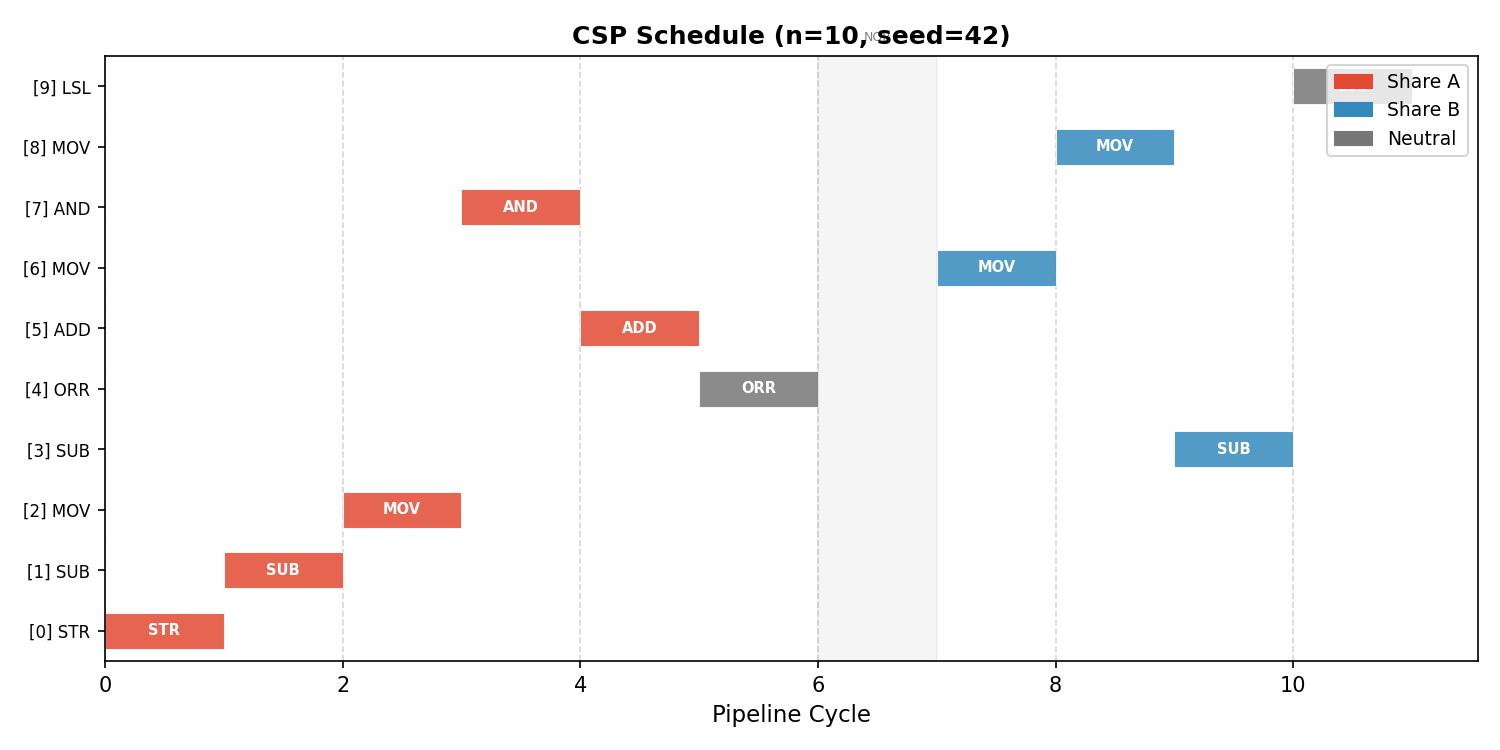
\includegraphics[width=\columnwidth]{../experiments/results/fig5_gantt_csp.png}
  \caption{Example schedule (Gantt chart) generated by the CSP solver for $n=10, k=3$. Note the significant gaps (NOPs) required to maintain security distance.}
  \label{fig:schedule}
\end{figure}

\subsection{MDP Reward-Shaping Ablation}
\label{sec:mdp-ablation}

The default reward shape ($-1$/cycle, $-10$/violation, $+50$/completion)
proved miscalibrated: at $n \in \{30, 50\}$ the cumulative cycle cost of
NOP injection exceeds the per-violation penalty, so the agent
\emph{rationally} drops NOPs and tolerates several SEC violations per
episode (rows marked $^{\dagger}$ in Table~\ref{tab:results_k3};
$E[L]$ up to $8.5$).
We re-ran the DQN at $n=10$ with the violation penalty rescaled to
$-100$ (script: \texttt{experiments/rerun\_mdp\_tuned.py}; full GPU
training, $5{,}000$ episodes per seed). Averaged over seeds
$\{42, 43, 44\}$, the tuned agent reaches $11.7 \pm 0.5$ cycles,
$1.67$ NOPs and $E[L] = 0.13$ with a $100\%$ valid rate
(row $^{\star}$): within $6\%$ of the CSP optimum and approaching the Bayesian
heuristic in expected leakage ($E[L] = 0.13$ vs $0.05$).. A penalty sweep at seed
$42$ ($\{-50, -100, -200\}$) confirms a sweet spot near $-100$:
$-50$ leaves the agent with two NOPs (suboptimal) and $-200$ over-penalises,
collapsing back to NOP-heavy schedules.

Based on these results, we redesign the DQN training strategy
to address two identified limitations: the single-block training
regime and the miscalibrated reward function.

\subsection*{Generalist Training}

The original setup trains one DQN per $(n, \text{seed})$ combination,
resulting in nine independent networks that each overfit to a single
instruction block. To change this, we train a \textit{single}
generalist DQN on a set of
$30\ \text{seeds} \times 3\ \text{sizes} = 90$ distinct blocks,
sampled uniformly at each episode. Test seeds $\{42, 43, 44\}$
are strictly excluded from the training set to prevent data
leakage, ensuring that the evaluation measures
generalisation rather than memorisation.

\subsection*{Normalised Reward Function}

The standard reward penalises each cycle by $-1$ and rewards
completion with $+50$, regardless of block size. This is
problematic for multi-block training: a block of $n=50$
accumulates far greater cycle penalties than $n=10$, producing
an inconsistent reward signal across sizes and biasing the
agent towards smaller blocks.

We introduce a size-normalised reward function,
\textit{shaped\_quality}:
\begin{align}
  r_{\text{cycle}}     & = -\frac{1}{n}                                                          \\
  r_{\text{place}}     & = +\frac{0.5}{n} \quad \text{(per instruction placed)}                  \\
  r_{\text{violation}} & = -\frac{P}{n}  \quad \text{(per security violation, } P = -100\text{)} \\
  r_{\text{done}}      & = +\frac{5n}{\text{total\_cycles}} \quad \text{(completion bonus)}
\end{align}

Each component addresses a specific weakness of the original design.
The per-cycle cost $-1/n$ and the per-placement bonus $+0.5/n$
keep the reward magnitude consistent across block sizes,
accelerating convergence in the multi-block setting.
The violation penalty $P = -100$, ten times stronger than in
the standard setup, aggressively discourages security constraint
violations — directly addressing the reward miscalibration
identified in Section~\ref{sec:mdp-ablation}. Finally, the completion
bonus $5n/\text{total\_cycles}$ rewards compact schedules:
it reaches its maximum of $5.0$ when no NOP is inserted,
and decreases proportionally with idle cycles, guiding the
agent towards the CSP optimum.
Table ~\ref{tab:generalist} contains the average results of the Generalist DQN. Generalist DQN achieves $100\%$ valid schedules, but $E[L]$ remains slightly higher than
Bayesian inference. This is a direct consequence of their
respective objectives: Bayesian explicitly minimises
$E[L]$ at each step via the CPT, while the DQN only penalises
hard SEC violations --- No difference between $\Delta t = 3$ or $\Delta t = 10$ cycles, as both satisfy the constraint.
\begin{table}[t]
  \centering
  \begin{tabular}{ccccc}
    \hline
    $n$ & Cycles ($\mu$) & NOPs ($\mu$) & Leakage$_E$ ($\mu$) & Wall time (s) \\
    \hline
    10  & 12.0           & 2.0          & 0.10                & 0.011         \\
    30  & 31.7           & 1.7          & 0.33                & 0.026         \\
    50  & 54.3           & 4.3          & 0.43                & 0.043         \\
    \hline
  \end{tabular}
  \caption{Generalist DQN benchmark results (mean over seeds 42, 43, 44), $k=3$.
    All schedules are valid (0 security violations).
    Wall time reflects inference only.}
  \label{tab:generalist}
\end{table}

%%table of average results for the new multi-block trained DQN 

%% ============================================================
\section{Qualitative Comparison}
\label{sec:qualitative}

\subsection{Strengths and Weaknesses}

\bayesHead{Bayesian Network Inference.}
\textit{Strengths}: Nuanced and realistic modeling of physical side-channel behavior. Instead of a hard binary cutoff $k$ which limits code density, the Bayesian approach permits densely packed instructions if their combined risk expectation falls below the threshold $\tau$. Extremely fast $O(n^2)$ inference during compilation.
\textit{Weaknesses}: It is a greedy heuristic that does not offer global makespan optimality. Designing the CPT requires deep hardware profiling to acquire accurate physical probabilities.

\cspHead{Constraint Satisfaction (CSP / OR-Tools).}
\textit{Strengths}: the declarative encoding is compact and easy to
extend (e.g.\ adding resource constraints such as register-file
pressure is a one-line model change); CP-SAT delivers \emph{proven
  optimal} solutions at $n = 50$ in $< 1$~s thanks to clause learning and
CDCL propagation; parallel workers give free speed-up on multi-core
machines.
\textit{Weaknesses}: although the algorithmic principles (CDCL,
two-watched literals, portfolio search) are well understood, the solver
remains operationally opaque --- pinpointing \emph{which} learned clause
forced a particular ordering requires dumping the proof log and replaying
the implication graph; encoding cross-product security constraints introduces
$O(|A| \cdot |B|)$ Boolean reification variables, which becomes the
dominant memory cost for large blocks.

\dqnHead{MDP / Deep Q-Network.}
\textit{Strengths}: once trained, inference is near-instantaneous
(${\sim}30$\,ms at $n=50$)); the fixed-size state/action feature representation is
block-size-independant, i.e.\ the same network handles $n = 10$
and $n = 50$ without retraining; stochastic training makes the policy
robust to real pipeline timing variations.
\textit{Weaknesses}: no optimality guarantee; training is long andcostly; reward shaping is delicate.

\subsection{Impact of Security Distance $k$}

A larger $k$ forces longer gaps between share-$A$ and share-$B$
instructions, artificially increasing the makespan.  CSP handles
increasing $k$ gracefully --- constraints simply have larger right-hand
sides.  The Bayesian greedy solver is also insensitive to $k$ as a hard
parameter: it continues to inject NOPs whenever the expected leakage
exceeds $\tau$, so its per-step cost is unchanged (only the total NOP
count grows).  For the MDP, a larger $k$ should be handled by adapting the
reward function accordingly. We believe that combining
penalty normalisation by $n$ with a violation penalty
proportional to $k$ (i.e.\ $P \propto k$) would allow the
DQN to remain robust in high-security regimes: larger $k$
forces more NOP insertions, increasing the cumulative cycle
cost, and a scaled penalty would preserve the relative
cost-benefit balance that drives valid schedule generation.
Due to time constraints and the significant training
cost, we focused our generalist training on $k=3$. This choice also
aligns with our CPT model, which assigns $P(L=1) = 0.00$ for
$\Delta t \geq 4$ cycles --- suggesting that $k=3$ provides
sufficient temporal separation under our leakage assumptions,
while $k=50$ constitutes an extreme stress-test.
\begin{figure}[h]
  \centering
  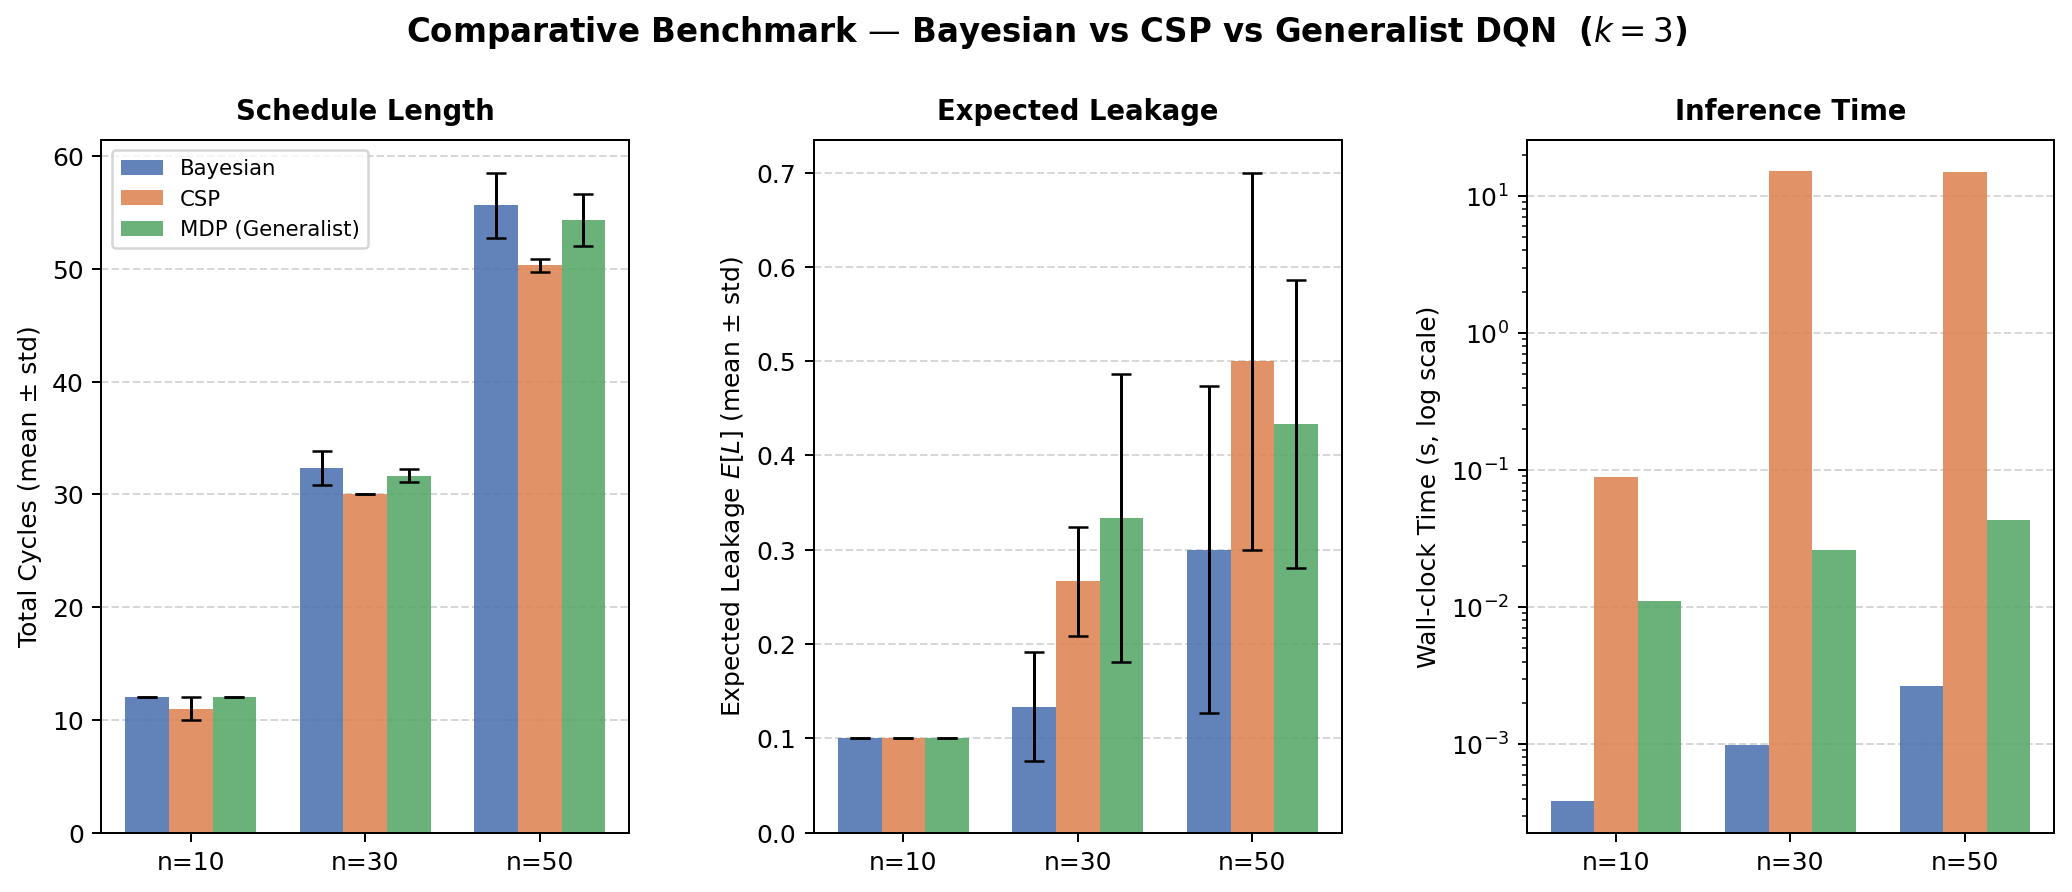
\includegraphics[width=\columnwidth]{../experiments/results/fig_comparison_all_correct.png}
  \caption{Comparative benchmark across all three solvers for $k=3$,
    averaged over seeds $\{42, 43, 44\}$. Error bars show
    $\pm 1$ standard deviation. Wall-clock time is shown on
    a log scale; MDP reflects inference only (training excluded).}
  \label{fig:comparison-all}
\end{figure}
\subsection{When to Prefer Each Approach}

\begin{preferbox}{bayesColor}
  \textbf{\textcolor{bayesColor}{Bayesian}}: when strict execution deadlines govern compiling, but physical trace leakage must remain beneath a certifiable risk threshold.
\end{preferbox}
\begin{preferbox}{cspColor}
  \textbf{\textcolor{cspColor}{CSP}}: the recommended choice for production use at any block size when binary cryptographic distance guarantees ($k$) are absolute mandatory constraints.
\end{preferbox}
\begin{preferbox}{dqnColor}
  \textbf{\textcolor{dqnColor}{MDP}} appropriate when inference speed is paramount
  (e.g.\ a JIT compiler), when hardware timing is genuinely
  stochastic (latency jitter, speculative execution), or when
  no calibrated leakage model is available --- requiring only
  a binary security constraint $|t_A - t_B| \geq k$ rather
  than a physically-motivated CPT
\end{preferbox}



%% ============================================================
\section{Conclusion}
\label{sec:conclusion}

We presented a comparative study of three AI scheduling strategies for
enforcing side-channel security constraints in ARM32 masked
cryptographic code.  Our main findings are: \newline
\textcolor{bayesColor}{Bayesian inference} offers a much more nuanced
trade-off than a rigorous threshold, successfully balancing statistical
leakage risk with code density at sub-millisecond cost; \newline
\textcolor{cspColor}{CP-SAT} is the most optimal combinatorial solver, returning provably optimal schedules at
$n=50$ within seconds; \newline
\textcolor{dqnColor}{DQN} provides near-instantaneous \emph{inference} after training, but is highly sensitive to reward shaping and training distribution design. Its ability to generalize depends on the diversity of the instruction blocks encountered during training.

Future work includes extracting direct CPT matrices from physical Cortex-M4
oscilloscopes, training DQN on higher security distances $k$
and stochastic training environments.
Another promising direction is a  hybrid CSP\,+\,RL
approach where the CSP provides a feasibility oracle for the agent.

%% ============================================================
\section{Reproducibility}
All source code, experiment scripts, Dockerfile, and detailed execution
instructions are available at:\\
\url{https://github.com/mordamed/arm-scheduler}

\noindent Please refer to the repository's \texttt{README.md} for the complete set of commands to build the Docker environment and reproduce all benchmarks and training procedures.

%% ============================================================
\bibliographystyle{aaai2026}
\bibliography{references}

\end{document}
